%%%%%%%%%%%%%%%%%%%%%%%%%%%%%%%%%%%%%%%%%%%%%%%%
%
% Strath PhD Thesis Template
%	by Jethro Browell [jethro.browell@strath.ac.uk]
%
%	Guidelines for thesis format, submission and content are found in
%	General and Course Regulations for Graduate and Postgraduate
%	Awards and Degrees, section 20.6.
%
%	Using .eps or .pdf is recomended to prduce high quality figures etc.
%
%	The Strathclyde logo can be found in other formats at www.strath.ac.uk.
%
%%%%%%%%%%%%%%%%%%%%%%%%%%%%%%%%%%%%%%%%%%%%%%%%

\documentclass[a4paper,oneside,11pt]{book}
\setcounter{secnumdepth}{3}
\usepackage{amsbsy}
\usepackage{amsmath}
\usepackage{amsfonts}
\usepackage{graphicx}
\usepackage{multirow}
\usepackage{mathrsfs}
\usepackage{color}
\usepackage[hidelinks]{hyperref}
\usepackage{cite}
\usepackage{enumitem}
\usepackage{epsfig}
\usepackage{caption}
\usepackage{subcaption}
\usepackage[strict]{changepage}

% Page Margins - Strath Requirement
\usepackage[left=4cm,right=2.5cm,top=2cm,bottom=4cm,includehead,includefoot,headheight=15pt]{geometry}

% Page Headers
\usepackage{fancyhdr}
\fancyhf{}
\renewcommand{\headrulewidth}{0pt} % optional
%\fancyhead[L]{\nouppercase{\leftmark} \hfill Section \nouppercase{\rightmark}}
\fancyhead[L]{\nouppercase{\leftmark}}
\cfoot{\thepage}
\pagestyle{fancy}

% Draft Watermark
\usepackage[draft=true,allpages=true,fontfamily=cmr,angle=90,scale=0.1,mark={\fboxsep=35pt\fboxrule=0pt\relax\fbox{-- DRAFT -- \today~--}},xcoord=-80,ycoord=-20]{draftmark}


% Line Spacing
%\def\baselinestretch{1.5} 
\usepackage{setspace}
\setstretch{1.5}


% Place UoS Logo on Title Page (this package modifies the "\maketitel" command.)
\usepackage{titling}


%%%%%%%%%%%%%%%%%%%%%%%%%%%%%%%%%%%%%%%%%%%%%%%%%%%%%%%%%%%%%%
\begin{document}
%%%%%%%%%%%%%%%%%%%%%%%%%%%%%%%%%%%%%%%%%%%%%%%%%%%%%%%%%%%%%%

\setcounter{chapter}{3}
\chapter{Complex Langevin dynamics of simple spherical aggregates}
Much of the calibration theory discussed in Chapter 2 assumes that the target particle in question is a single sphere, one who's scattering and motion is easily computed. However, while working with dense colloidal suspensions, one often ends up trapping more than one sphere. Li and Arlt \cite{Li2008} studied the case of two microspheres trapped in a single OT and found that multiple trapped beads could be mistaken for a single trapped bead with altered trap stiffness. Theoretical studies on the case of two trapped microspheres by Xu \textit{et.al.} \cite{Xu2005} employed a ray-optics based model to show that the two trapped beads are brought into physical contact with each other by optical forces and they also calculated the axial equilibrium positions of the two trapped beads as a function of their size. Experiments in \cite{Praveen2016} confirmed that the two trapped beads indeed experience different trap stiffnesses in the vicinity of the same potential well. There are further discussions looking into the dynamics of a whole host of asymmetrically shaped particles \cite{Loudet2014, ShengHua2005, Chetana2022}, their results all showing that predicting the behaviour an arbitrary shaped particle comes with great difficulty due to the fact that the optical force is dependent on a greater number of variables such as orientation and size factors.

In this chapter we consider how the addition of a second sphere into an optical trap can radically effect its dynamics, to the extent that one can no longer rely on typical calibration techniques to characterise the interactions.

\section{Positional and Orientational dependence of Trapping forces}
If we wanted to start from first principles and determine the trap strength on our target particle the first step would be to locate the harmonic traps relative to the trap focus. The methodology for computing optical forces has been covered extensively for a number of different trapping conditions \cite{RanhaNeves2019}, so it is relatively easy to compute the trapping force and determine where a simple sphere would be located relative to focal point of the laser. We can do so because the optical force is only dependent on the particle's relative position. If we instead consider a asymmetric dimer for example we see just by inverting the particle then a secondary harmonic trap can be found below the focus.

\begin{figure}[h]
	\centering
	\begin{subfigure}{.475\linewidth}
		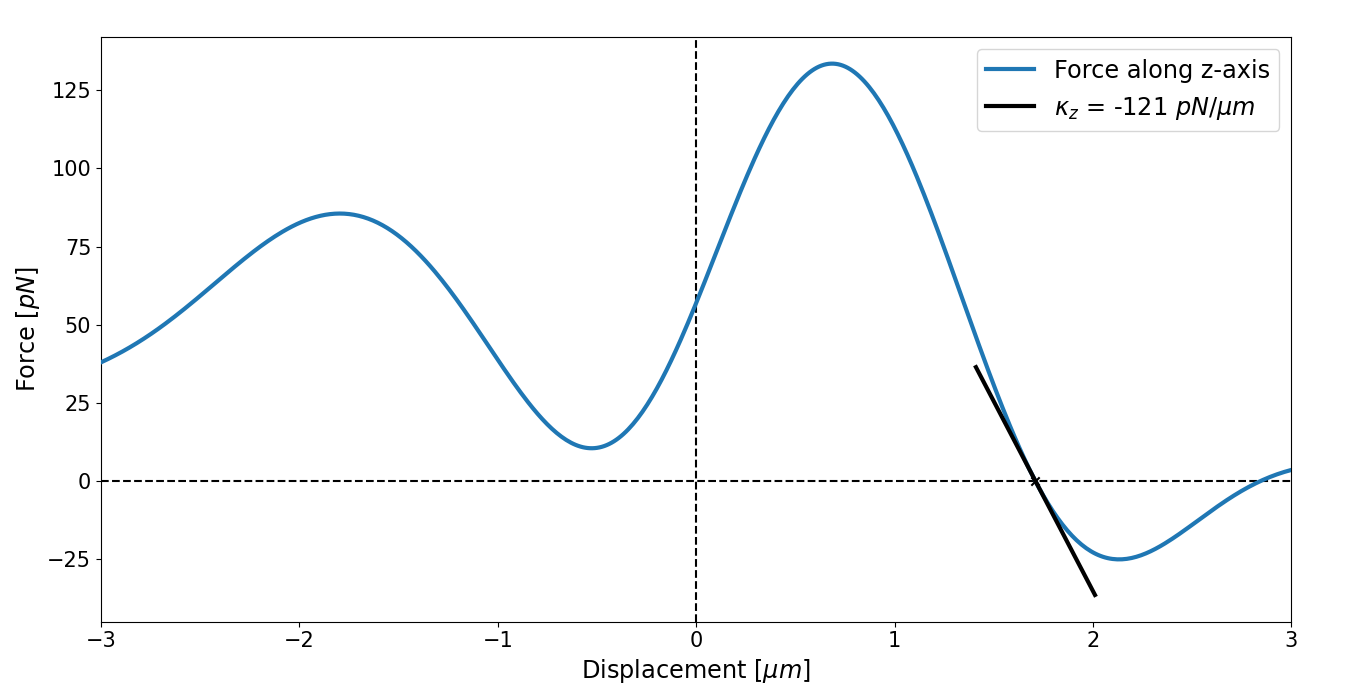
\includegraphics[width=\linewidth]{lam=2_theta=0.png}
		\caption{}
		\label{lam=2}
	\end{subfigure}\hfill % <-- "\hfill"
	\begin{subfigure}{.475\linewidth}
		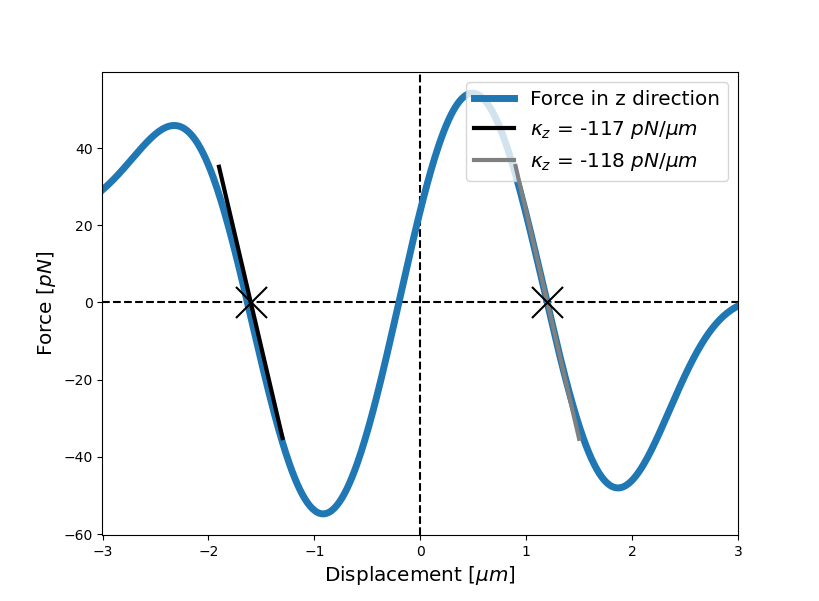
\includegraphics[width=\linewidth]{lam=2_theta=180.png}
		\caption{}
		\label{lam=2_inverted}
	\end{subfigure}\hfill % <-- "\hfill"
	\medskip
	\begin{subfigure}{.475\linewidth}
		\centering
		\raisebox{65pt}[0pt][0pt]{\makebox{}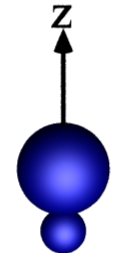
\includegraphics[width=0.3\linewidth, keepaspectratio]{theta=0.png}}
		\label{large over small}
	\end{subfigure}
	\begin{subfigure}{.475\linewidth}
		\centering
		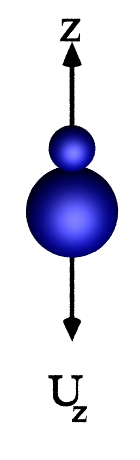
\includegraphics[width=0.3\linewidth, keepaspectratio]{theta=180.png}
		\label{small_over_large}
	\end{subfigure}
	\caption{Plots of force vs displacement of the point of the contact of the spheres (µm) for the case of a dimer of size ratio 2. (a) is the case where the smaller sphere is orientated with the beam propagation direction. (b) is the inverted case, smaller sphere oriented against the propagation direction. Renders to visualise the dimer orientation are shown below each plot The black lines on each force-curve is a linear fit with the slope being reported as the trap stiffness in the legend.}
\end{figure}

We can see that the trap below the focus is comparable in strength to above the focus, however the difference in the transverse strength is far more noticeable. As shown below in Fig~\ref{fig:transverse_force}, the dimer's orientation and relative position significantly changes the force curve; not only is the trap wider when inverted but the trap stiffness is increased. This highlights one of the challenges involved with studying asymmetric particles, even though its a simple enough process to trap them they maybe characterised very differently depending on their relative position and orientation towards the trap. This can have a significant impact on rheological studies - or attempting to probe any local property - as the variance in trap strength can result in large errors over repeated measurements. 
\begin{figure}
	\centering
	\label{fig:transverse_force}
	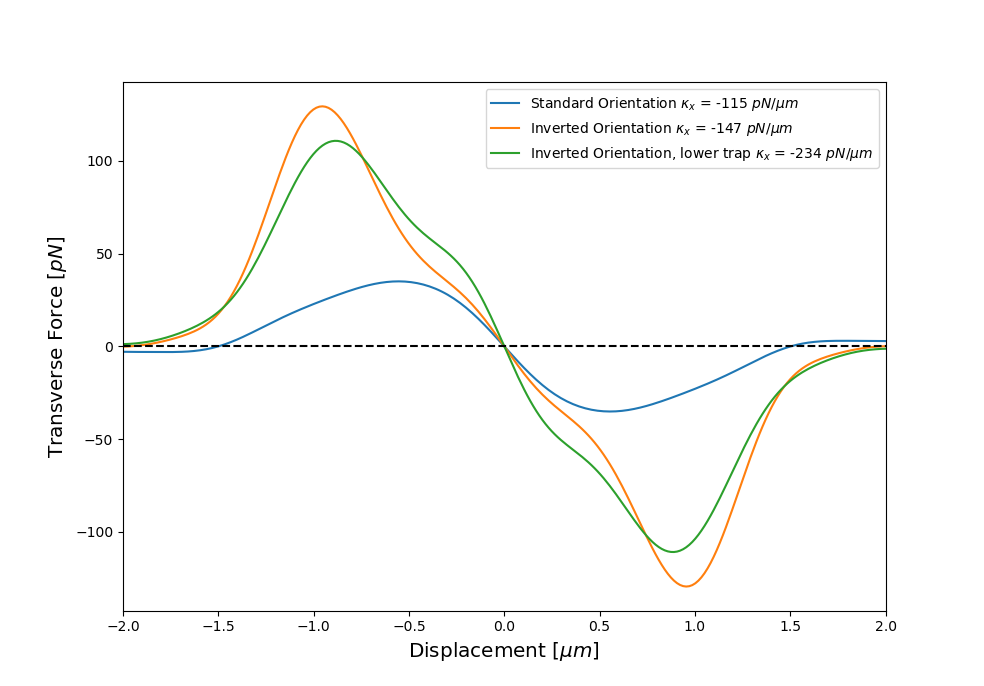
\includegraphics[width=0.67\linewidth]{transverse_force.png}
	\caption{Plots of force vs displacement of the point of the contact of the spheres (µm) for the case of a dimer of size ratio 2 while being displaced in the transverse plane. With the blue curve representing the force response for a dimer in its standard orientation, orange being the inverted case, and green the same case but placed below the focus.}
\end{figure}

For completeness the harmonic traps were located for dimers across a range of size ratios - from $a_1/a_2 = 1$ to $a_1/a_2=10$ - while also recording the trap stiffness for each trap. As $a_2$ decrease the dimer begins to approximate a single homogenous sphere - at least in terms of location and trap strength. However, for intermediate sized dimers (between $a_1/a_2 = 1.1$ to $a_1/a_2=4$), a second harmonic trap appeared below the trapping focus. Previous work using the ray-optics model have confirmed even in the case that two spheres begin separated the electric field will align the molecules as such that they make contact and are trapped together about a single trapping position \cite{Xu2005}. Furthermore it has been shown through proper manipulation of the Gaussian or Bessel beam modes that any number of trapping potentials can be developed \cite{Shahabadi2020}. This result however, is the first example of an orientation dependent trapping situation using only a $TEM_00$ beam. 

\begin{figure}[h]
	\centering
	\begin{subfigure}{0.85\linewidth}
		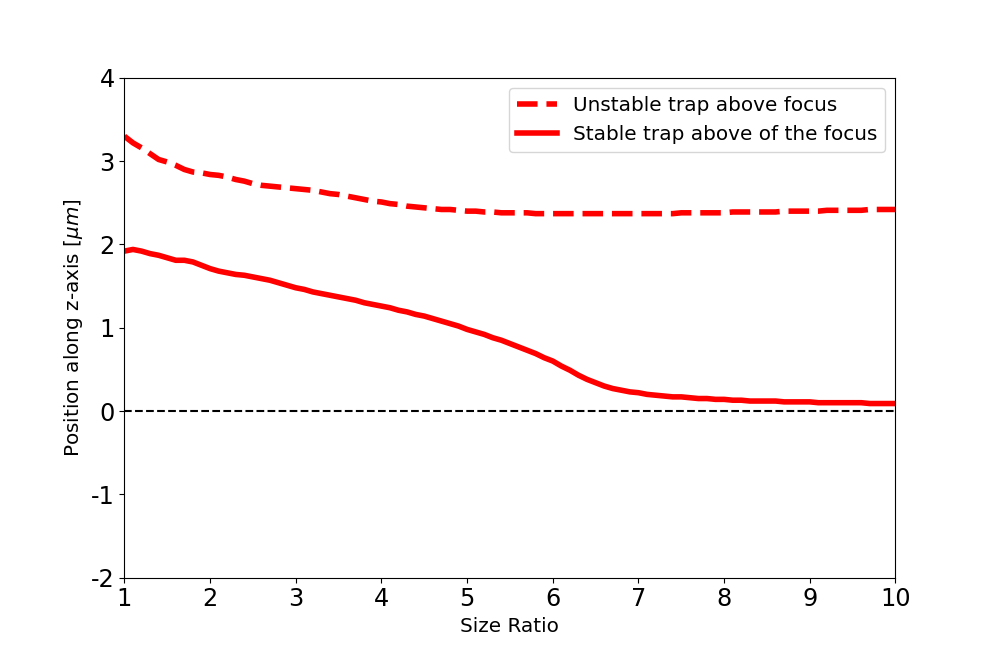
\includegraphics[width=\linewidth]{Equillibrium_positions.png}
		\caption{}
		\label{eq_pos}
	\end{subfigure}\hfill % <-- "\hfill"
	\medskip
	\begin{subfigure}{0.85\linewidth}
		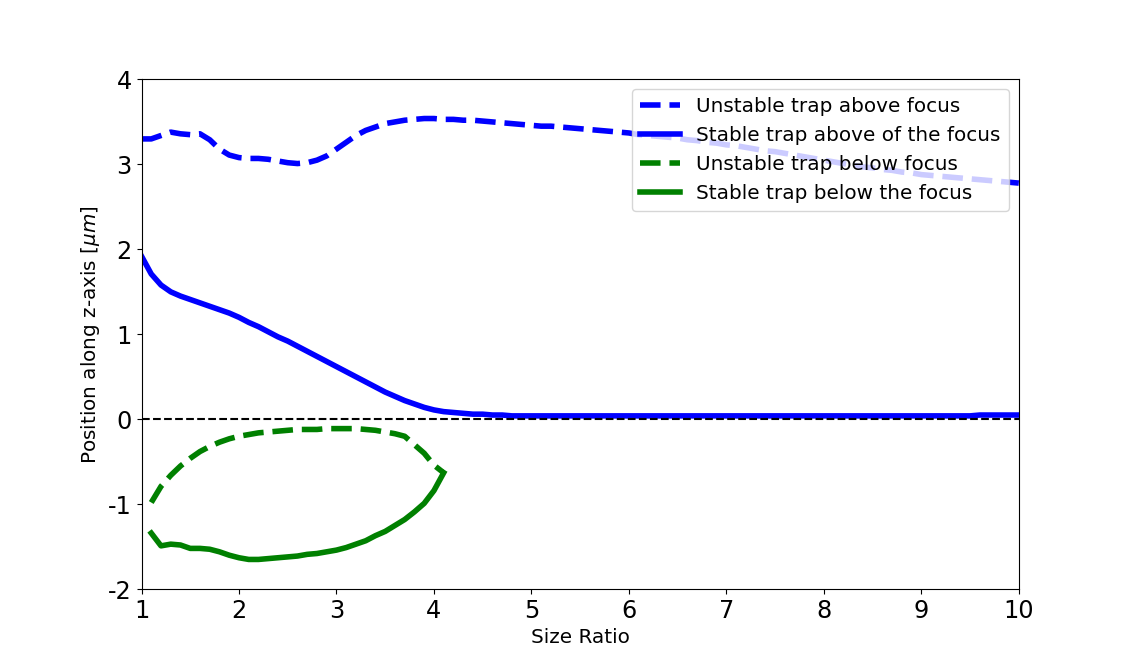
\includegraphics[width=\linewidth]{Equillibrium_positions_inverted.png}
		\caption{}
		\label{eq_pos_inverted}
	\end{subfigure}
	\caption{Equilibrium positions of optically trapped dimers with varying size ratio, dotted lines represent unstable traps whereas solid lines represent stable trapping positions. (a) shows that dimers with their smaller sphere orientated away from the focus have an expected single trapping position. (b) shows that when the same dimer is inverted $180^\circ$ there are now stable traps along the beam axis, one below the focus and one above the focus.}
\end{figure}

This was only seen when the dimer is orientated with the smaller sphere above the larger sphere, when the dimer is flipped then the force curve only intersects the x-axis once, regardless of size ratio. More noteworthy is that in this orientation the dimer’s equilibrium position reaches its limit at a smaller size ratio; before it took a size ratio of 1:4 to achieve a final equilibrium position whereas now the second sphere needed to shrink until it was 1/7th of the first sphere’s size before the equilibrium position settled. This would suggest by having a second sphere behind the first, the momentum transfer from the beam to the dimer is diminished resulting in a weaker force pushing against the dimer as it sits within the trap. And when the dimer is flipped this shielding is lost and so both beads are being pushed by the beam.

Computing the equilibrium positions when a dimer is aligned with the electric field is relatively trivial as the orientational torque is minimised (see Eq.\ref{eq:opt_torque}), meaning once trapped the dimer is unlikely to change orientation enough to escape the trap. However, that does not rule out the possibility that there is a stable orientation that is not strictly vertical, in fact most experimental work with symmetric dimers will trap them lying perpendicular to the beam direction \cite{Ahn2018}. Unlike before where we can simply find the trap by varying the dimer's vertical position its instead more prudent to run a multitude of smaller simulations at a variety of starting positions and orientations. An example for a dimer of size ratio 2 is shown below:

\begin{figure}
	\centering
	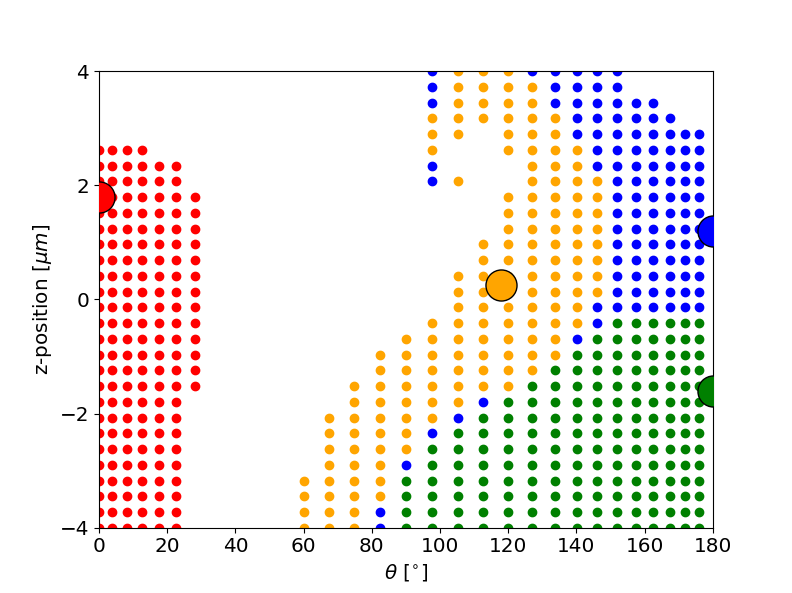
\includegraphics[width=0.75\linewidth]{off_axis_trap.png}
	\caption{Trajectory map of simulations ran using a dimer of size ratio 2 with a laser power of 500 mW. The stable points are indicated by the larger spheres and the starting conditions are colour coded to match the stable point they end up in.}
\end{figure}

Interestingly the trap strength of the these off-axis traps are similar in magnitude to the vertically aligned traps, but when the laser power is lowered (to ~5 mW) the traps become metastable resulting in the dimer escaping from after some random time in the trap. 
\bibliographystyle{ieeetran}
\bibliography{thesis_bib}

\end{document}